\documentclass[tikz,border=15pt]{standalone}
\usetikzlibrary{arrows.meta, positioning}

\begin{document}
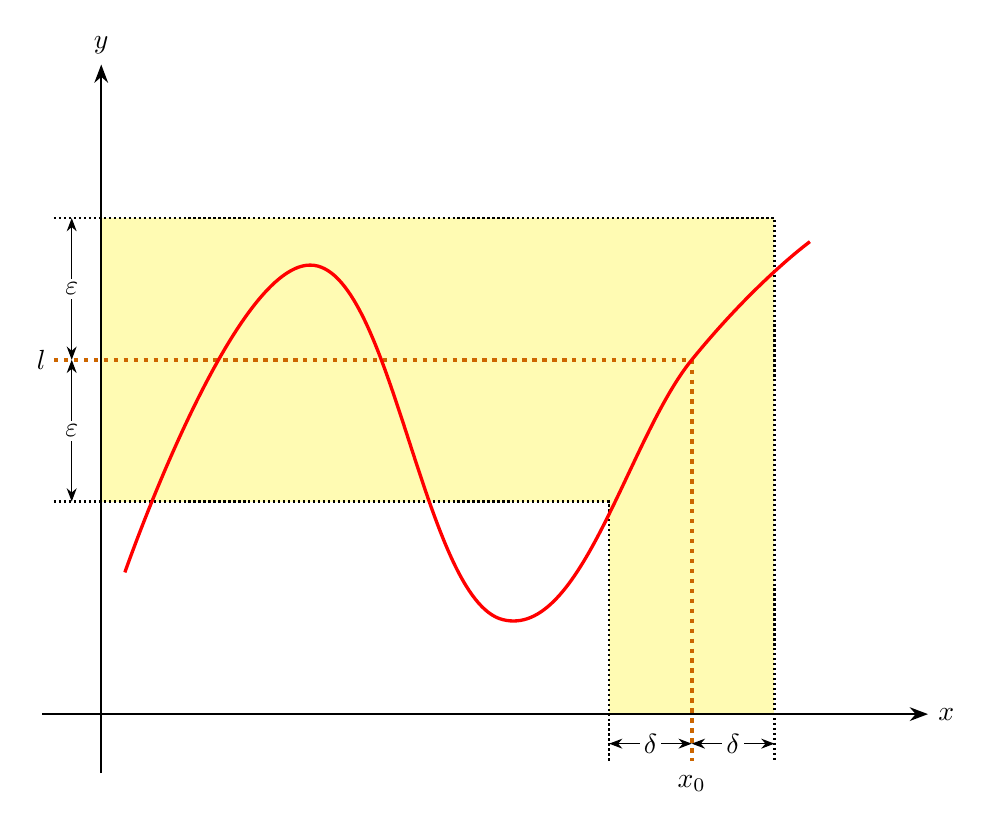
\begin{tikzpicture}[>=Stealth, scale=1.5]

    % 定义核心参数，方便统一调整比例
    \def\xO{5}       % x_0 的横坐标
    \def\yL{3}       % l 的纵坐标
    \def\del{0.7}    % \delta 的区间宽度
    \def\eps{1.2}    % \varepsilon 的区间宽度

    % 1. 绘制高亮填充区域 (浅黄色)
    % 水平方向的 \varepsilon 矩形框 (从 y 轴一直延伸到 x_0 + \delta)
    \fill[yellow!30] (0, \yL-\eps) rectangle (\xO+\del, \yL+\eps);
    % 垂直方向的 \delta 矩形框 (从 x 轴上方补全剩余部分)
    \fill[yellow!30] (\xO-\del, 0) rectangle (\xO+\del, \yL-\eps);

    % 2. 绘制辅助虚线
    % 上边界虚线 (l + \varepsilon)
    \draw[thick, densely dotted] (-0.4, \yL+\eps) -- (\xO+\del, \yL+\eps) -- (\xO+\del, -0.4);
    % 下边界虚线 (l - \varepsilon)
    \draw[thick, densely dotted] (-0.4, \yL-\eps) -- (\xO-\del, \yL-\eps) -- (\xO-\del, -0.4);
    % 中心参考线 (l 和 x_0)，使用橙黄色加粗点线以作区分
    \draw[ultra thick, dotted, orange!80!black] (-0.4, \yL) -- (\xO, \yL) -- (\xO, -0.4);

    % 3. 绘制坐标轴
    \draw[thick, ->] (-0.5, 0) -- (7, 0) node[right] {$x$};
    \draw[thick, ->] (0, -0.5) -- (0, 5.5) node[above] {$y$};

    % 4. 绘制函数曲线
    % 使用平滑曲线使其自然穿过边界框的三个关键交叉点
    \draw[very thick, red, smooth, tension=0.75] plot coordinates {
        (0.2, 1.2)
        (1.8, 3.8)
        (3.4, 0.8)
        (\xO, \yL)
        (6, 4)
    };

    % 5. 标注 y 轴相关文本与箭头
    \node[left=8pt] at (-0.2, \yL) {$l$};
    % 绘制 \varepsilon 的指示箭头，使用 fill=white 防止文字与坐标轴打架
    \draw[<->] (-0.25, \yL) -- node[fill=white, inner sep=1.5pt] {$\varepsilon$} (-0.25, \yL+\eps);
    \draw[<->] (-0.25, \yL-\eps) -- node[fill=white, inner sep=1.5pt] {$\varepsilon$} (-0.25, \yL);

    % 6. 标注 x 轴相关文本与箭头
    \node[below=10pt] at (\xO, -0.2) {$x_0$};
    % 绘制 \delta 的指示箭头
    \draw[<->] (\xO-\del, -0.25) -- node[fill=white, inner sep=1.5pt] {$\delta$} (\xO, -0.25);
    \draw[<->] (\xO, -0.25) -- node[fill=white, inner sep=1.5pt] {$\delta$} (\xO+\del, -0.25);

\end{tikzpicture}
\end{document}